% !TEX root = ./main.tex
\begin{figure}[h]
    \centering
    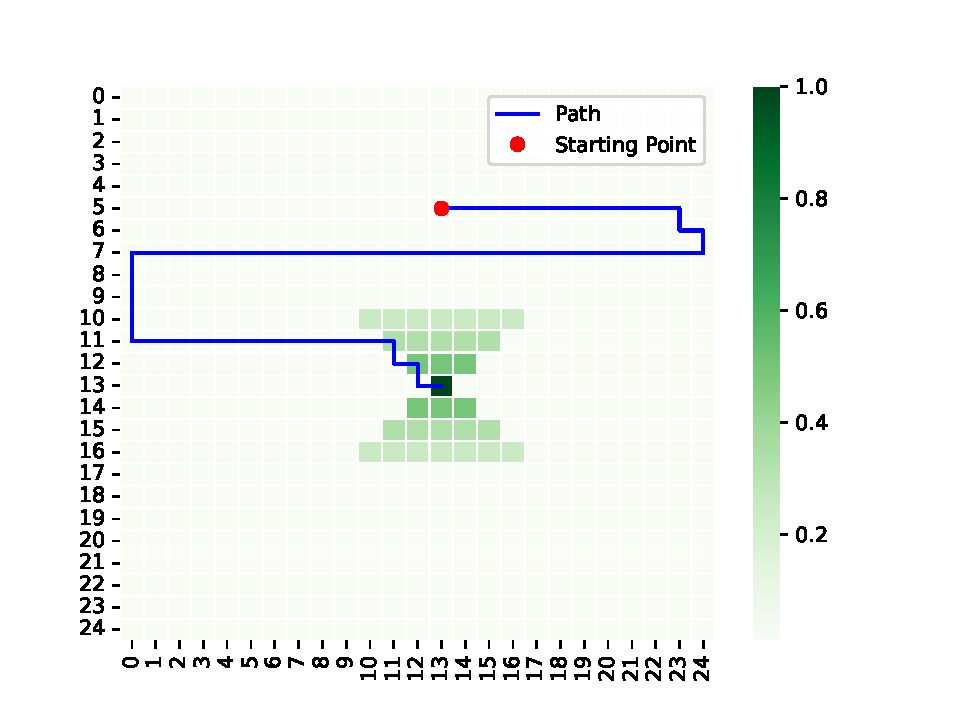
\includegraphics[width=0.95\textwidth]{path_1.pdf}
    \vspace{-5mm}
    \caption{Plot of a trajectory generated using Infotaxis starting from a random location of door and agent within the $25 \times 25$ grid.
    The heatmap shows the ground truth, i.e.~the probability of obtaining a measurement of $z=1$.
    This example shows a particularly ``lucky'' search, where the agent obtained a positive measurement whenever near the door.}
    \label{fig:path1}
\end{figure}
\begin{figure}[h]
    \centering
    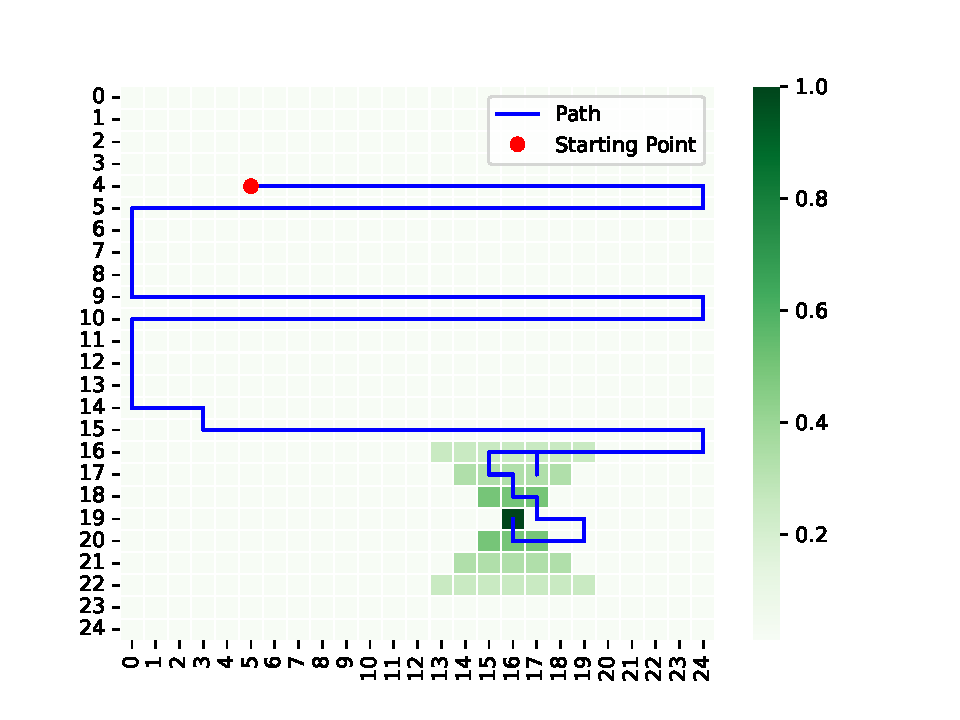
\includegraphics[width=0.95\textwidth]{path_2.pdf}
    \vspace{-5mm}
    \caption{Plot of a trajectory generated using Infotaxis starting from a random location of door and agent within the $25 \times 25$ grid.
    The heatmap shows the ground truth, i.e.~the probability of obtaining a measurement of $z=1$.
    This example shows how the implementation of the algorithm seems to show different behaviours at the left and right edges of the grid, 
    going vertically for more steps whenever at the left edge. This is most possibly due to some coding error\ldots 
    But I think it's a happy accident because this speeds up walking through the grid considerably!}
    \label{fig:path2}
\end{figure}
\begin{figure}[h]
    \centering
    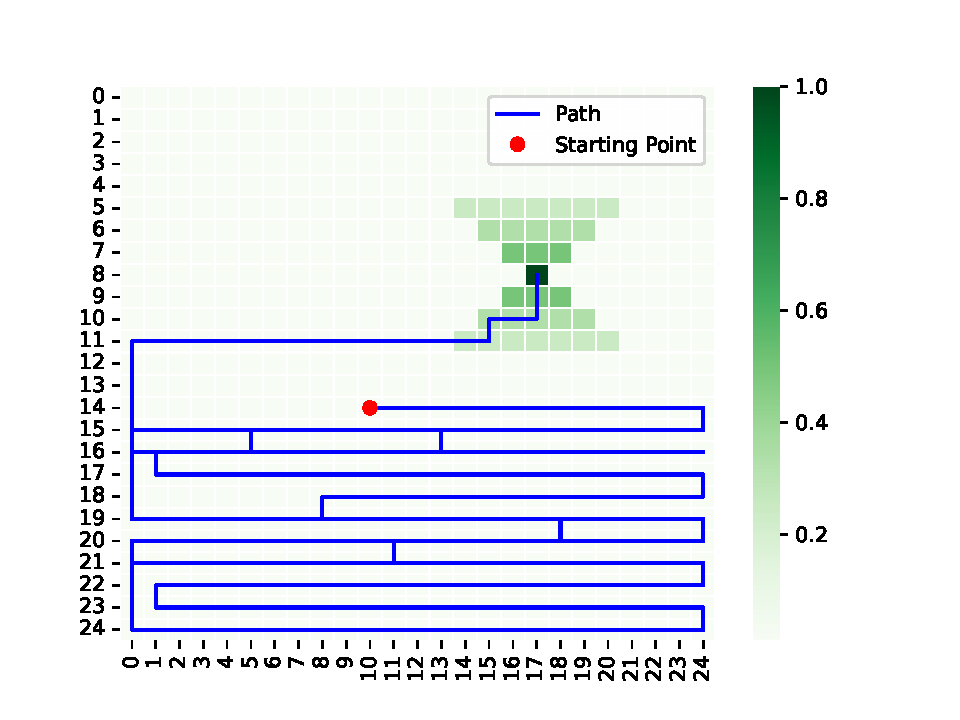
\includegraphics[width=0.95\textwidth]{path_3.pdf}
    \vspace{-5mm}
    \caption{Plot of a trajectory generated using Infotaxis starting from a random location of door and agent within the $25 \times 25$ grid.
    The heatmap shows the ground truth, i.e.~the probability of obtaining a measurement of $z=1$. 
    This one is a bit unlucky, because it went to the bottom of the map where it didn't find anything.}
    \label{fig:path3}
\end{figure}
\begin{figure}[h]
    \centering
    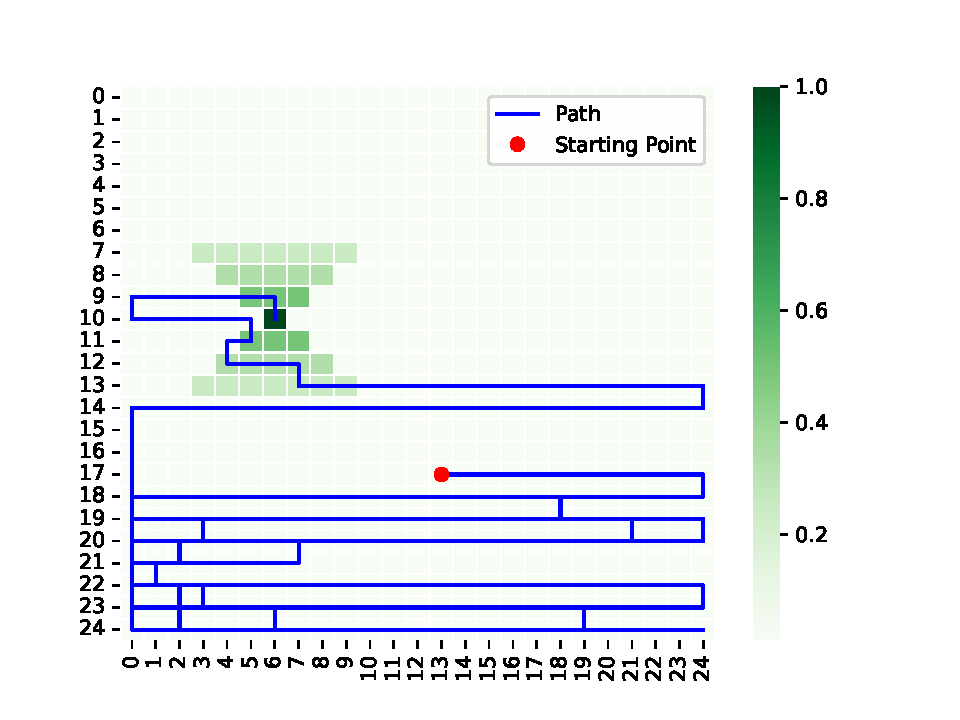
\includegraphics[width=0.95\textwidth]{path_4.pdf}
    \vspace{-5mm}
    \caption{Plot of a trajectory generated using Infotaxis starting from a random location of door and agent within the $25 \times 25$ grid.
    The heatmap shows the ground truth, i.e.~the probability of obtaining a measurement of $z=1$. 
    Here, the agent manages to find the door, but walks away again (probably due to measuring $z=0$ near the door).}
    \label{fig:path4}
\end{figure}